\documentclass[a4paper]{scrartcl}

% font/encoding packages
\usepackage[utf8]{inputenc}
\usepackage[T1]{fontenc}
\usepackage{lmodern}
\usepackage[ngerman]{babel}
\usepackage[ngerman=ngerman-x-latest]{hyphsubst}

\usepackage{amsmath, amssymb, amsfonts, amsthm}
\usepackage{array}
\usepackage{stmaryrd}
\usepackage{marvosym}
\allowdisplaybreaks
\usepackage[output-decimal-marker={,}]{siunitx}
\usepackage[shortlabels]{enumitem}
\usepackage[section]{placeins}
\usepackage{float}
\usepackage{units}
\usepackage{listings}
\usepackage{pgfplots}
\pgfplotsset{compat=1.12}
\usepackage{tikz}
\usetikzlibrary{arrows,automata}

\newtheorem*{behaupt}{Behauptung}
\newcommand{\gdw}{\Leftrightarrow}
\newcommand{\dif}{\ \mathrm{d}}
\newcommand{\N}{\mathbb{N}}
\newcommand{\prob}{\mathbb{P}}
\newcommand{\cov}{\operatorname{Cov}}
\newcommand{\e}{\mathbb{E}}
\newcommand{\var}{\operatorname{Var}}
\newcommand{\corr}{\operatorname{Corr}}

\usepackage{fancyhdr}
\pagestyle{fancy}

\lstset{%
    frame=single,
    numbers=left,
    keepspaces,
    language=R,
    title=Listing: \lstname,
}

\def \blattnr {4}

\lhead{Stochastik 2 - Blatt {\blattnr}}
\rhead{Florian Abt, Lennart Braun, Sascha Schulz}
\cfoot{\thepage}


\title{Stochastik 2 für Informatiker}
\subtitle{Blatt {\blattnr} Hausaufgaben}
\author{
    Florian Abt (6524404), \\
    Lennart Braun (6523742), \\
    Sascha Schulz (6434677)
}
\date{zum 10. November 2015}

\begin{document}
\maketitle

\begin{enumerate}[label=\bfseries \blattnr.\arabic*]
    \item
    $G(V,E) \to G'(V', E')$ mit $V' = V$, $E' = E\setminus\{(f,f)\}$

    \begin{minipage}{0.25\textwidth}
    \centering
    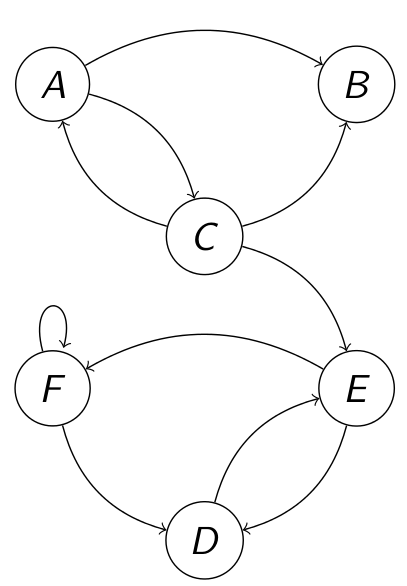
\includegraphics[width=0.75\textwidth]{assets/graph-vorher.png}     
    \end{minipage}
    \begin{minipage}{0.01\textwidth}
    \centering
    $\to$     
    \end{minipage}
    \begin{minipage}{0.24\textwidth}
     \centering
     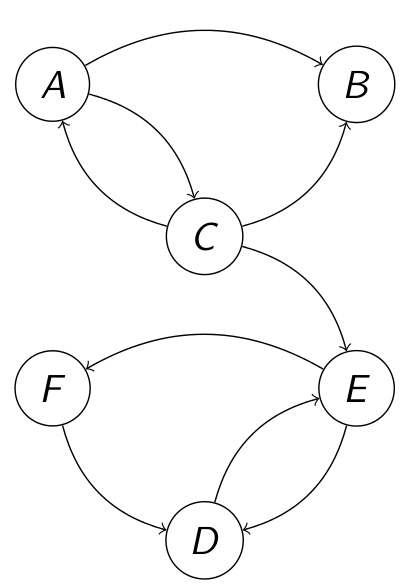
\includegraphics[width=0.75\textwidth]{assets/graph-nachher.png}
    \end{minipage}
    \begin{minipage}{0.5\textwidth}
     \begin{equation*}
	A' = \begin{pmatrix}
	     0 & 1 & 1 & 0 & 0 & 0 \\
	     0 & 0 & 0 & 0 & 0 & 0 \\
	     1 & 1 & 0 & 0 & 1 & 0 \\
	     0 & 0 & 0 & 0 & 1 & 0 \\
	     0 & 0 & 0 & 1 & 0 & 1 \\
	     0 & 0 & 0 & 1 & 0 & \textbf{0}
	    \end{pmatrix}
     \end{equation*}
    \end{minipage}
    
    \begin{minipage}{0.5\textwidth}
      \begin{equation*}
	H' = \begin{pmatrix}
	     0 & \frac12 & \frac12 & 0 & 0 & 0 \\
	     0 & 0 & 0 & 0 & 0 & 0 \\
	     \frac13 & \frac13 & 0 & 0 & \frac13 & 0 \\
	     0 & 0 & 0 & 0 & 1 & 0 \\
	     0 & 0 & 0 & \frac12 & 0 & \frac12 \\
	     0 & 0 & 0 & \textbf{1} & 0 & \textbf{0}
	    \end{pmatrix}
     \end{equation*}
    \end{minipage}
    \begin{minipage}{0.5\textwidth}
     \begin{equation*}
	S' = \begin{pmatrix}
	     0 & \frac12 & \frac12 & 0 & 0 & 0 \\
	     \frac16 & \frac16 & \frac16 & \frac16 & \frac16 & \frac16 \\
	     \frac13 & \frac13 & 0 & 0 & \frac13 & 0 \\
	     0 & 0 & 0 & 0 & 1 & 0 \\
	     0 & 0 & 0 & \frac12 & 0 & \frac12 \\
	     0 & 0 & 0 & \textbf{1} & 0 & \textbf{0}
	    \end{pmatrix}
     \end{equation*}
    \end{minipage}
    
    $G' = \alpha S' + (1-\alpha)E$ mit $\alpha = \frac 9{10}$:
    
    \begin{equation*}
	G' = \begin{pmatrix}
	     \frac{1}{60} & \frac{28}{60} & \frac{28}{60} & \frac{1}{60} & \frac{1}{60} & \frac{1}{60} \\
	     \frac{10}{60} & \frac{10}{60} & \frac{10}{60} & \frac{10}{60} & \frac{10}{60} & \frac{10}{60} \\
	     \frac{19}{60} & \frac{19}{60} & \frac{1}{60} & \frac{1}{60} & \frac{1}{60} & \frac{19}{60} \\
	     \frac{1}{60} & \frac{1}{60} & \frac{1}{60} & \frac{1}{60} & \frac{55}{60} & \frac{1}{60} \\
	     \frac{1}{60} & \frac{1}{60} & \frac{1}{60} & \frac{28}{60} & \frac{1}{60} & \frac{28}{60} \\
	     \frac{1}{60} & \frac{1}{60} & \frac{1}{60} & \frac{55}{60} & \frac{1}{60} & \frac{1}{60}
	    \end{pmatrix}
     \end{equation*}
     
     Dies führt laut Wolfram-Alpha für den Eigenwert 1 zum Eigenvektor:
     
    \begin{equation*}
	v_1 \approx (0.19804, 0.287159, 0.220891, 1.83373, 1.78213, 1)
     \end{equation*}
     
     Wir teilen jeden Eintrag durch die Summe, damit ein stochastischer Vektor entsteht:
     
     \begin{equation*}
      \Rightarrow \pi \approx (0.0372119, 0.0539575, 0.0415057, 0.34456, 0.334864, 0.187901)
     \end{equation*}
     
     Somit ergibt sich für G' die Rangfolge: D, E, F, B, C, A. 
     
     Vergleichen wir dies mit der Rangfolge, die auf Basis von G errechnet wurde (F, D, E, B, C, A)
     sehen wir, dass F in G' zwei Rangplätze verloren hat. Das entfernen des Selbst-Links hatte also 
     drastische Folgen.
    
    \item
        \begin{enumerate}
            \item
                Es sei $Y \sim \text{U}(0,1)$.
                \begin{behaupt}
                    \begin{equation*}
                        \e[Y] = \frac{1}{2}
                    \end{equation*}
                \end{behaupt}
                \begin{proof}
                    \begin{equation*}
                        \begin{split}
                            \e[Y]
                            &= \int_{-\infty}^\infty y \cdot f_Y(y) \dif y \\
                            &= \int_0^1 y \cdot 1 \dif y \\
                            &= \left[ \frac{1}{2}y^2 \right]_0^1 \\
                            &= \frac{1}{2} - 0 = \frac{1}{2}
                        \end{split}
                    \end{equation*}
                \end{proof}

            \item
                Es sei $Y \sim \text{Exp}(\lambda)$.
                \begin{behaupt}
                    \begin{equation*}
                        \e[Y] = \frac{1}{\lambda}
                    \end{equation*}
                \end{behaupt}
                \begin{proof}
                    Verwendung der Dichte
                    \begin{equation*}
                        \begin{split}
                            \e[Y]
                            &= \int_{-\infty}^\infty y \cdot f_Y(y) \dif y \\
                            &= \int_0^\infty y \cdot
                                \lambda e^{-\lambda y} \dif y \\
                            &\stackrel{a=a+b-b}{=} \int_0^\infty 
				\left(y \cdot \lambda e^{-\lambda y} 
				  - 1 \cdot e^{-\lambda y} \right) \dif y 
				+ \int_0^\infty e^{-\lambda y} \dif y \\
                            &= \lim_{a \to \infty} \left[ -y e^{-\lambda y}
                                \right]_0^a
                                + \lim_{b \to \infty} \left[ -\frac{1}{\lambda} e^{-\lambda y}
                                \right]_0^b \\
                            &= \lim_{b \to \infty} \left( -b \cdot 
                                e^{-\lambda \cdot b} \right)
                                - \left( - 0 \cdot 
                                e^{-\lambda \cdot 0} \right)
                                + \lim_{a \to \infty}
                                \left( -\frac{1}{\lambda} e^{-\lambda \cdot a}
                                \right) - \left( -\frac{1}{\lambda}
                                e^{-\lambda \cdot 0} \right) \\
                            &= \lim_{b \to \infty} \left( - \frac{b}{e^{\lambda b}} \right) - 0 + 0 - \left(-\frac1\lambda \right) \\
                            &\stackrel{l'Hospital}{=} \lim_{b \to \infty} \left( - \frac{1}{\lambda e^{\lambda b}} \right) + \frac1\lambda 
                             = \frac{1}{\lambda}
                        \end{split}
                    \end{equation*}
                    Verwendung der Verteilung
                    \begin{equation*}
                        \begin{split}
                            \e[Y]
                            &= \int_0^\infty 1 - F_Y(y) \dif y \\
                            &= \int_0^\infty 1 - (1 - e^{-\lambda y}) \dif y \\
                            &= \int_0^\infty e^{-\lambda y} \dif y \\
                            &= \left[ -\frac{1}{\lambda}e^{-\lambda y}
                                 \right]_0^\infty \\
                            &= \lim_{x \to \infty} \left(
                                 -\frac{1}{\lambda}e^{-\lambda \cdot x} \right) 
                                 -\left( -\frac{1}{\lambda}e^{-\lambda \cdot 0}
                                 \right) \\
                            &= 0 - \left( -\frac{1}{\lambda} \right)
                             = \frac{1}{\lambda}
                        \end{split}
                    \end{equation*}
                \end{proof}

            \item
                Sei $Z$ eine Zufallsvariable mit der Verteilungsfunktion
                $F_Z \colon \mathbb{R} \to [0,1]$:
                \begin{equation*}
                    F_Z(z) =
                    \begin{cases}
                        1 - \alpha e^{-\lambda z} , & z \geq 0 \\
                        0 , & z < 0 \\
                    \end{cases}
                    \text{ für }
                    \alpha \in [0,1]
                \end{equation*}
                \begin{behaupt}
                    \begin{equation*}
                        \e[Z] = \frac{\alpha}{\lambda}
                    \end{equation*}
                \end{behaupt}
                \begin{proof}
                    \begin{equation*}
                        \begin{split}
                            \e[Z]
                            &= \int_0^\infty 1 - F_Z(z) \dif z \\
                            &= \int_0^\infty \alpha e^{-\lambda z} \dif z \\
                            &= \alpha \int_0^\infty e^{-\lambda z} \dif z \\
                            &= \alpha \cdot \frac{1}{\lambda}
                             = \frac{\alpha}{\lambda}
                        \end{split}
                    \end{equation*}
                \end{proof}

        \end{enumerate}

    \item 
        \begin{enumerate}
            \item
                Die Zufallsvariable $Y$ sei mit Parameter $\lambda$ verteilt:
                $Y \sim \text{Exp}(\lambda)$.
                \begin{behaupt}
                    Es gilt $\prob(Y > y) = e^{-\lambda y}$ für $y \geq 0$.
                \end{behaupt}
                \begin{proof}
                    \begin{equation*}
                        \prob(Y > y)
                        = 1 - \prob(Y \leq y)
                        = 1 - F_Y(y)
                        = 1 - (1 - e^{-\lambda y})
                        = e^{-\lambda y}
                    \end{equation*}
                \end{proof}

                \begin{behaupt}
                    Die Exponentialverteilung ist gedächtnislos:
                    Es gilt
                    \begin{equation*}
                        \prob(Y > s + t\ |\ Y > s) = \prob(Y > t)
                        \text{ für }
                        s,t \geq 0
                        \text{ .}
                    \end{equation*}
                \end{behaupt}
                \begin{proof}
                    \begin{equation*}
                        \begin{split}
                            \prob(Y > s + t\ |\ Y > s)
                            &= \frac{\prob(Y > s+t, Y > s)}{\prob(Y > s)} \\
                            &= \frac{\prob(Y > s+t)}{\prob(Y > s)} \\
                            &= \frac{e^{-\lambda (s+t)}}{e^{-\lambda s}} \\
                            &= e^{-\lambda t} \\
                            &= \prob(Y > t)
                        \end{split}
                    \end{equation*}
                \end{proof}
                
                Diese Eigenschaft wird als Gedächtnislosigkeit bezeichnet, da
                die Wahrscheinlichkeit für einen Wert s+t lediglich abhängig von
                der Distanz zum nächst kleineren Ereignis s ist, alle vorherigen
                Ereignisse sind für die Wahrscheinlichkeit irrelevant. Dies kann
                als Analogie zur Gedächtnislosigkeit bei einer DTMC betrachtet werden.

            \item
                Es seien $Y_1, \dotsc, Y_n$ unabhängig mit $Y_i \sim
                \text{Exp}(\lambda_i)$ für $i = 1, \dotsc, n$.
                \begin{behaupt}
                    $\min\{Y_1, \dotsc, Y_n\} \sim Exp(max\{\lambda_1, \dotsc, \lambda_n\})$.
                \end{behaupt}
                \begin{proof}
		    Sei $\min\{Y_1, \dotsc, Y_n\} = Y_k \sim Exp(\lambda_k)$.
		    Damit bleibt zu zeigen: Für welches $\lambda_i$ wird das zugehörige $Y_i$ minimal?
		    
		    Wir gehen davon aus dass $F_{Y_1}(y) < F_{Y_2}(y)$ für $y>0$.
                    \begin{equation*}
                        \begin{split}
                            \Rightarrow 1 - \frac1{e^{-\lambda_1y}} &< 1 - \frac1{e^{-\lambda_2y}} \\
                            \Rightarrow - \frac1{e^{-\lambda_1y}} &< - \frac1{e^{-\lambda_2y}} \\
                            \Rightarrow \frac1{e^{-\lambda_1y}} &> \frac1{e^{-\lambda_2y}} \\
                            \Rightarrow e^{-\lambda_2y} &> e^{-\lambda_1y} \\
                            \Rightarrow -\lambda_2y &> -\lambda_1y \\
                            \Rightarrow \lambda_2 &< \lambda_1 \\
                        \end{split}
                    \end{equation*}
                    
                    Somit gilt: $F_{Y_1}(y) < F_{Y_2}(y) \Rightarrow \lambda_2 < \lambda_1 \\$ und folglich
                    $\min\{Y_1, \dotsc, Y_n\} \sim Exp(\max\{\lambda_1, \dotsc, \lambda_n\})$.
                \end{proof}

            \item

        \end{enumerate}
   
\end{enumerate}


\end{document}
